\documentclass[10pt,twoside,french,a4paper]{article}

\usepackage[utf8]{inputenc}
\usepackage[T1]{fontenc}
\usepackage[french]{babel}
\usepackage[top=2cm,bottom=2cm,left=2cm,right=2cm]{geometry}
\usepackage{amsmath,mathtools,amssymb}
\usepackage{tabularx,array,diagbox}
\usepackage{graphicx}
\usepackage{listings}
\usepackage{caption}
\usepackage{footnote}

\lstset{language=PostScript,
  morekeywords={
    hsbw,
    hmoveto,
    vlineto,
    rrcurveto,
    endchar,
    callsubr,
    vhcurveto,
    hvcurveto,
    return},
  captionpos=b,
  frame=single}

\title{TIPE : Quantité d'encre utilisée par une fonte d'écriture}
\author{Clément Guidi}

\begin{document}

\begin{center}
  \LARGE \textbf{TIPE : Quantité d'encre utilisée par une fonte d'écriture} \\ Rapport final
\end{center}

\section{Préambule}

Ce TIPE vise à étudier la consommation d'encre des différentes fontes courament utilisées, pour déterminer dans quelle mesure il peut être avantageux d'en utiliser une en particulier.

Sur un ordinateur, les glyphes de ces fontes ont une représentation mathématique sous forme d'équations paramétrées, que l'on exploite pour calculer leurs aires.

On fournit une interprétation graphique des programmes développés \textit{via} l'interface graphique de Caml.

\section{Introduction}

Le travail réalisé a tout d'abord consisté à convertir et traiter les fichiers de fontes pour les manipuler avec Caml Light.

Une étude mathématique des cubiques de Bézier décrivant les glyphes a permis de mettre en place une méthode de calcul efficace des aires des glyphes, en accord avec le principe de l'algorithme récursif de De Casteljau.

Il a fallu normaliser et pondérer les aires calculées, pour obtenir des valeurs concernant des situations précises.

On a enfin pû donner une représentation graphique des caractéristiques des glyphes que l'on a identifiées.

\section{Corps principal}

\subsection{Modalités d’action}

\noindent \textbf{Obtention de données exploitables}

On a comparé les fontes suivantes :

\begin{itemize}

\item
  Arial

\item
  Comic Sans MS

\item
  Courier New

\item
  DejaVu Sans

\item
  Garamond

\item
  Times

\end{itemize}

\medskip

Les fichiers de ces fontes sont au format TrueType (\textsc{ttf}) ou OpenType (\textsc{otf}). Le logiciel \emph{fontforge} permet de les convertir au format PostScript Type 1 (\textsc{pfb}).

L'utilitaire \emph{t1disasm} convertit ensuite le \textsc{pfb} en \textsc{asm}, lisible par Caml Light.

\medskip

On a sélectionné les caractères suivants :

\begin{itemize}

\item
  Les lettres minuscules, non accentuées (de \emph{a} à \emph{z})

\item
  Les lettres capitales, non accentuées (de \emph{A} à \emph{Z})

\item
  Les chiffres (de \emph{0} à \emph{9})

\item
  Certains signes de ponctuation : \textbf{.} \textbf{,} \textbf{!} \textbf{?} \textbf{:} \textbf{;} ainsi que \textbf{'} \textbf{(} \textbf{)}

\end{itemize}

La description de ces caractères a été isolée manuellement dans les fichiers \textsc{asm} produits.

\medskip

Le reste de la programmation a été réalisé avec le langage Caml.

\pagebreak

\noindent \textbf{Traitement des données}

La description d'un glyphe au format \textsc{asm} se présente sous la forme :

\begin{lstlisting}[title={\fbox{Extrait de la description du glyphe de \emph{i} en Garamond}}]
  /i {
    24 245 hsbw
    42 565 hmoveto
    13 -6 vlineto
    ...
    0 45 5 49 4 41 rrcurveto
    8 callsubr
    closepath
    endchar
  } ND
\end{lstlisting}

\medskip

La description d'un glyphe est donnée dans le langage PostScript : la syntaxe est postfixée, les arguments sont relatifs (au point courant).

\medskip

\begin{itemize}

\item[$\rhd$]
  \textbf{hsbw} est ici ignoré.

\item[$\rhd$]
  \textbf{hmoveto} est une application partielle de \textbf{rmoveto}, qui déplace le point courant -- horizontalement ici.

\item[$\rhd$]
  \textbf{vlineto} est une application partielle de \textbf{rlineto}, qui déplace le point courant en traçant une ligne droite -- verticalement ici.
  
\item[$\rhd$]
  \textbf{rrcurveto} est au c\oe ur de ce \textsc{tipe} car c'est l'instruction de tracé d'une cubique de Bézier.

  Ces dernières sont des courbes paramétrées, caractérisées par quatre points de contrôle. Deux de ces points ($P_{000}$, $P_{111}$)  indiquent les deux extrémités de la courbe, les deux autres ($P_{001}$, $P_{011}$) orientent les demi-tangentes aux extrémités.
  
  Si on note les points de contrôle
  $
  \quad P000 = \begin{pmatrix}x_0\\y_0\end{pmatrix}
    \quad P001 = \begin{pmatrix}x_1\\y_1\end{pmatrix}
      \quad P011 = \begin{pmatrix}x_2\\y_2\end{pmatrix} 
        \quad P111 = \begin{pmatrix}x_3\\y_3\end{pmatrix}
          $,
          
          la courbe est paramétrée par :
          
          \[
          \forall t \in [0,1] \quad 
          \begin{cases}
            x(t) = x_0 (1-t)^3 + 3 x_1 (1-t)^2 t + 3 x_2 (1-t) t^2 + x_3 t^3 \\
            y(t) = y_0 (1-t)^3 + 3 y_1 (1-t)^2 t + 3 y_2 (1-t) t^2 + y_3 t^3
          \end{cases}
          \]

          \begin{figure}[h]
            \begin{center}
              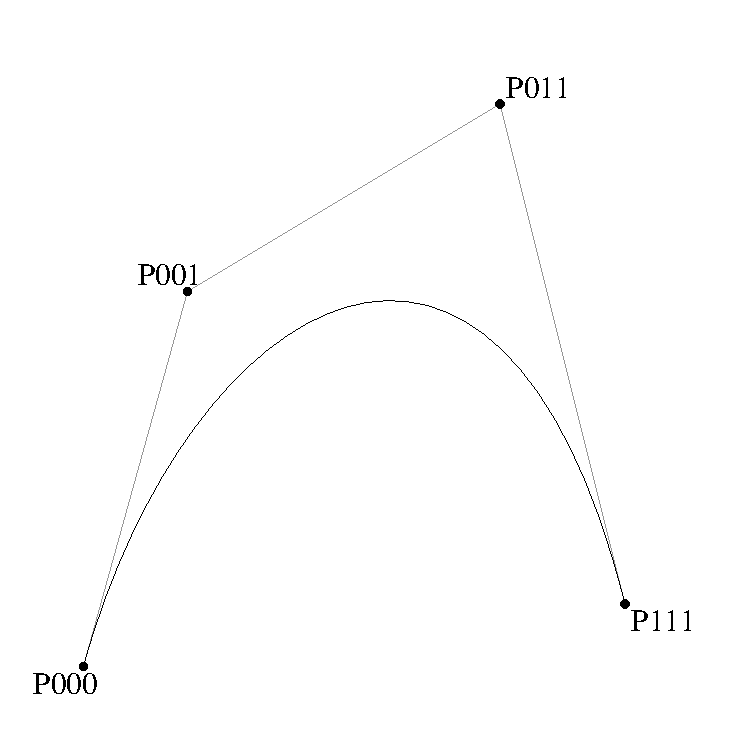
\includegraphics[width=10cm]{Ressources/pdf/f1.pdf}
              \caption{Exemple d'une courbe de Bézier (en noir)}
            \end{center}
          \end{figure}
          
        \item[$\rhd$]
          \textbf{callsubr} appelle une séquence préprogrammée -- ici le point du \emph{i}, avec les instructions précédentes. Elle est destinée à être utilisée dans la description de plusieurs glyphes, et est décrite par :

          \begin{lstlisting}[title={\fbox{Définition de la sous-routine \no 8 en Garamond}}]
            dup 8 {
              -28 22 -22 28 vhcurveto
              29 22 22 28 hvcurveto
              29 -22 22 -29 vhcurveto
              -28 -22 -22 -29 hvcurveto
              closepath
              return
            } NP
          \end{lstlisting}

        \item[$\rhd$]
          \textbf{closepath} et \textbf{endchar} permettent de fermer le glyphe avec des lignes droites.
          
\end{itemize}

\medskip

Un fichier \textsc{asm} est lu puis enregistré en Caml Light comme liste de chaînes de caractères.
Un premier parcours est réalisé pour formater les instructions et leurs arguments, et remplacer les sous-routines par leur description.
On peut ensuite effectuer des calculs sur la liste traitée.

\medskip

\noindent \textbf{Méthode de calcul}

Comme on l'a vu, un glyphe est composé de segments et de courbes de Bézier.

\begin{figure}[h]
  \begin{center}
    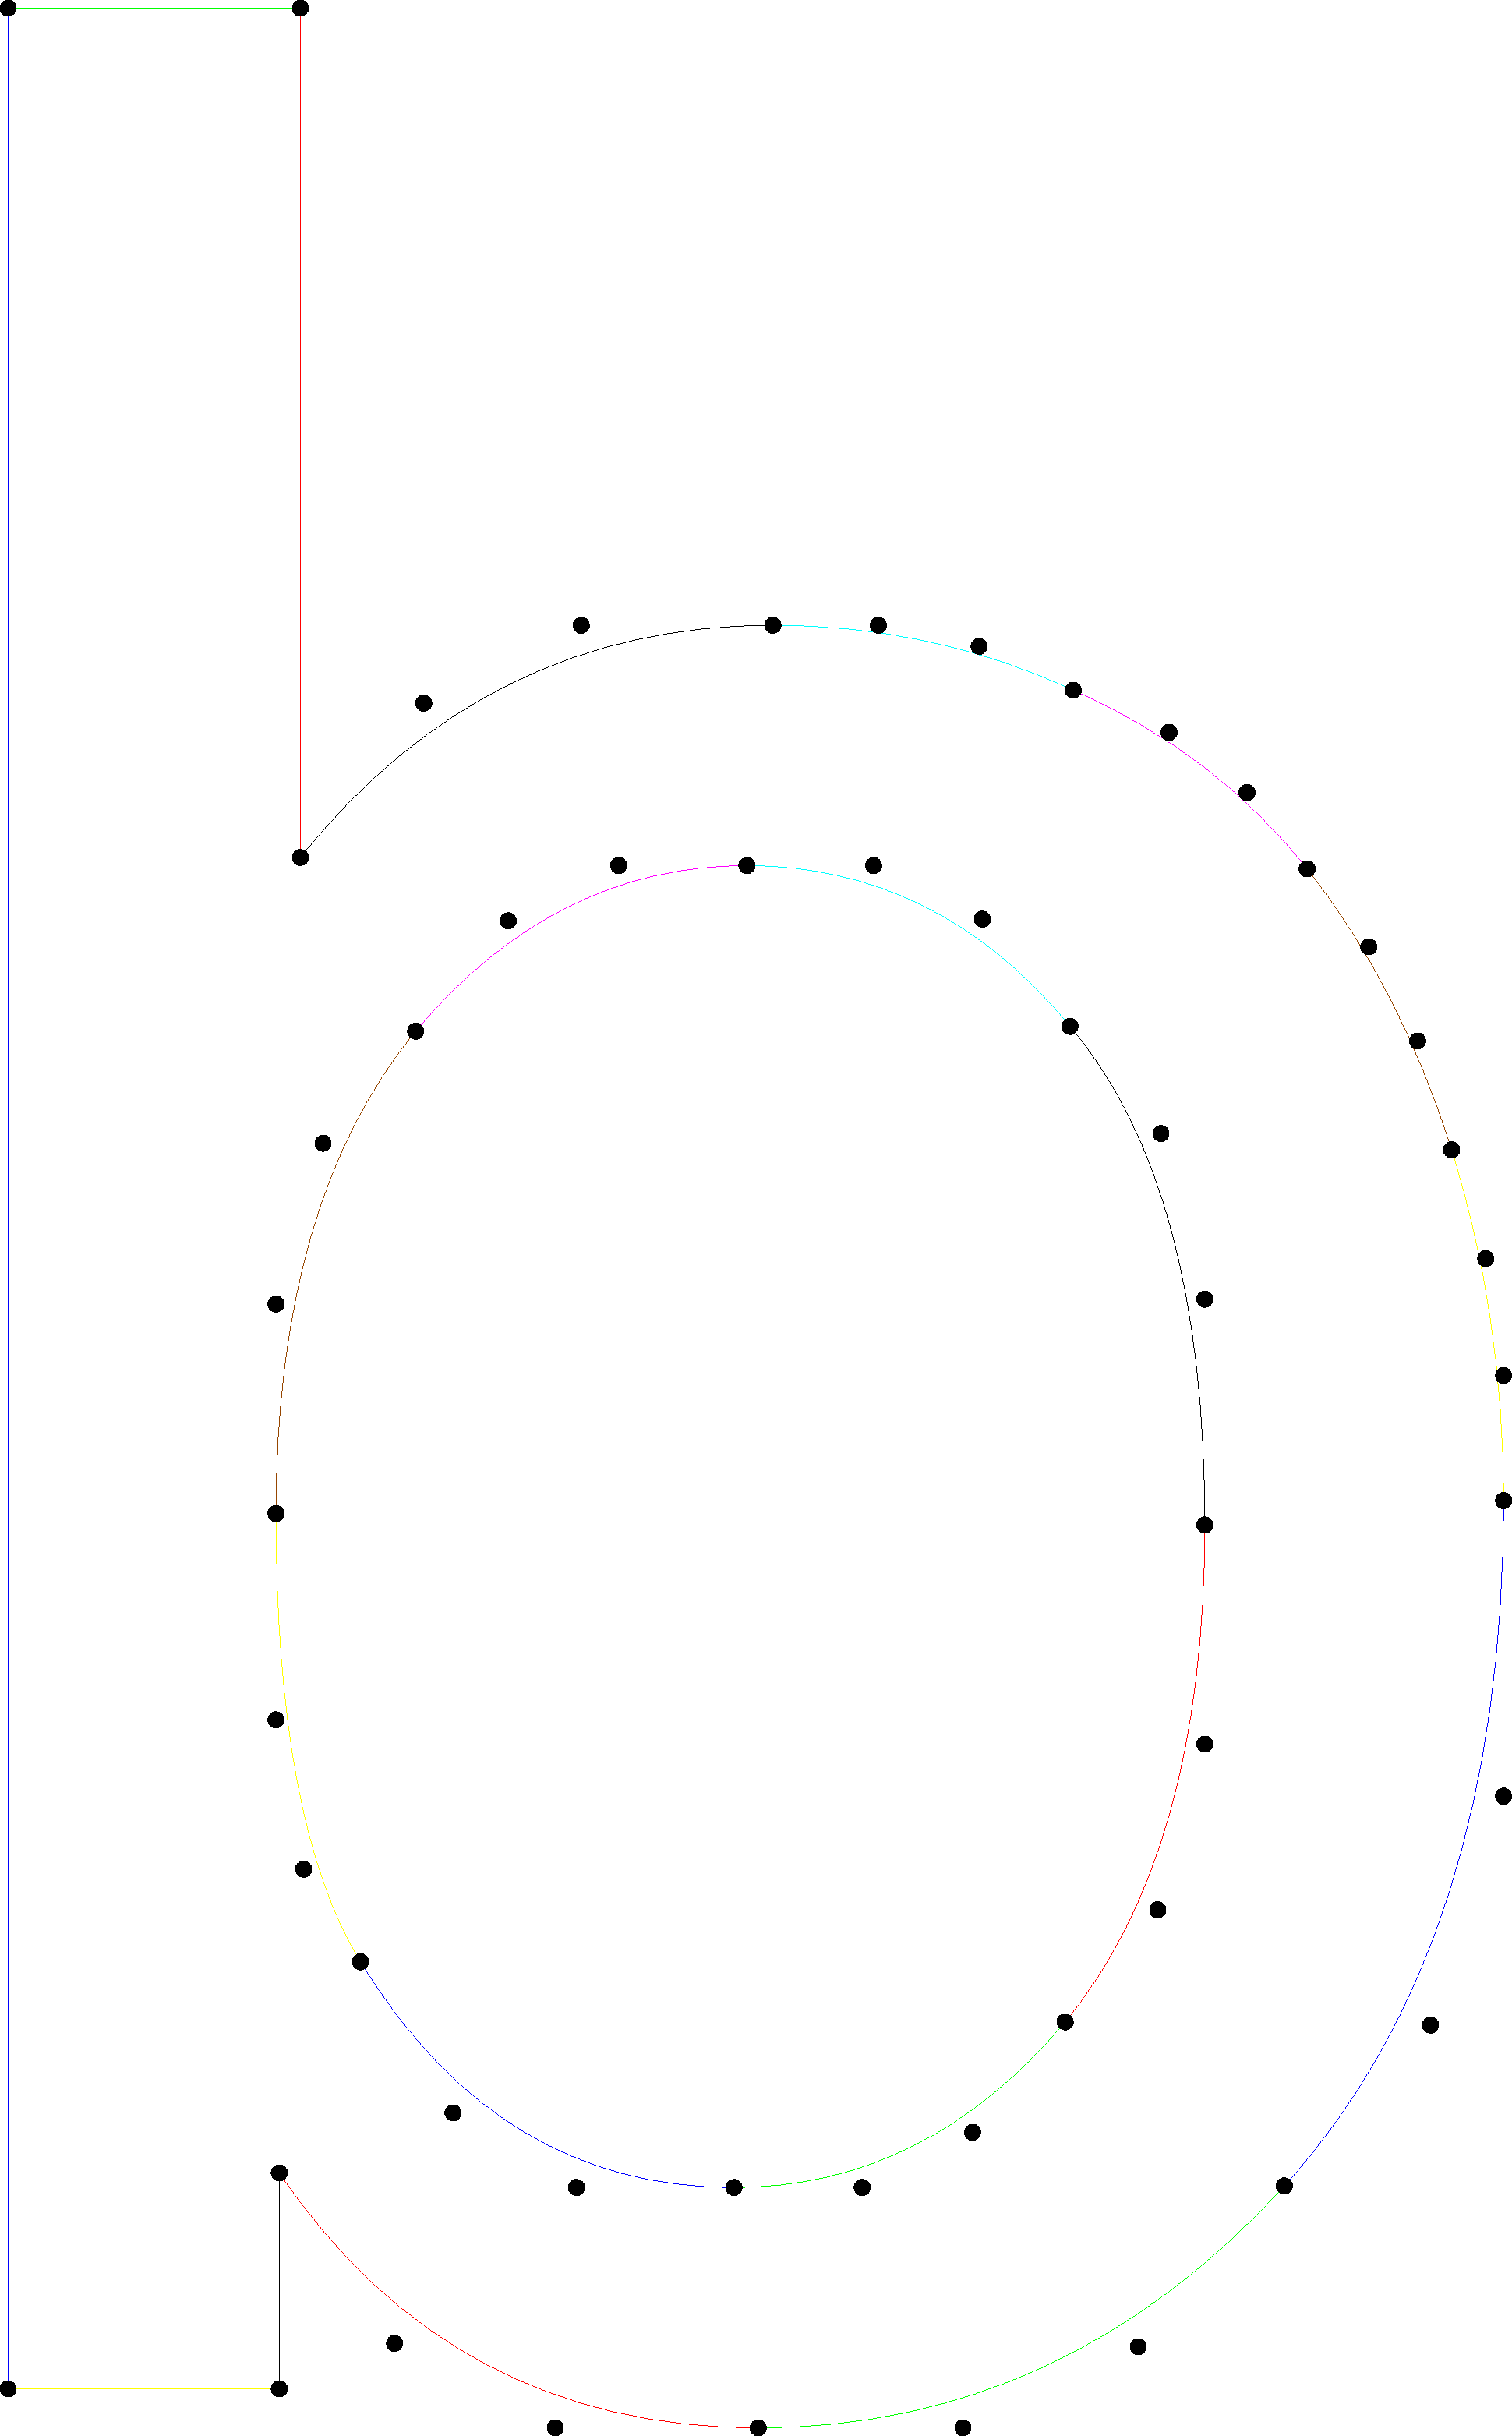
\includegraphics[height=12cm]{Ressources/pdf/b2.pdf}
    \caption{Décomposition du glype de \emph{b} en Arial\\En noir, les points de contrôle}
  \end{center}
\end{figure}

\pagebreak

La formule de Green-Riemann donne l'aire $\mathcal{A}$ d'une portion de plan enclose par un contour paramétré fermé et orienté $\mathcal{C}$ :

\[ \mathcal{A} = \frac{1}{2} \int_{\mathcal{C}} (x \mathrm{d}y - y \mathrm{d}x) \]

\medskip

Un glyphe est alors parcouru récursivement, les aires de ses sections étant sommées pour obtenir l'aire totale.

\medskip

Pour pouvoir comparer les fontes, les  aires sont calculées par rapport à l'aire d'un carré de côté la hauteur du glyphe de \emph{x} -- c'est une convention.
La méthode pour la calculer et de calculer la « bounding box » du glyphe (rectangle contenant la lettre, voir \textsc{Figure} \ref{Bounding box b}). On a mis en place cette démarche pour tout les glyphes.

L'exemple du \emph{b} en Arial est parlant. La \textsc{Figure} \ref{Bounding box b} illustre comment chaque section contribue à agrandir la « bounding box » (de la même couleur). La première « bounding box » calculée est la rouge en bas à gauche.

\begin{figure}[h]
  \begin{center}
    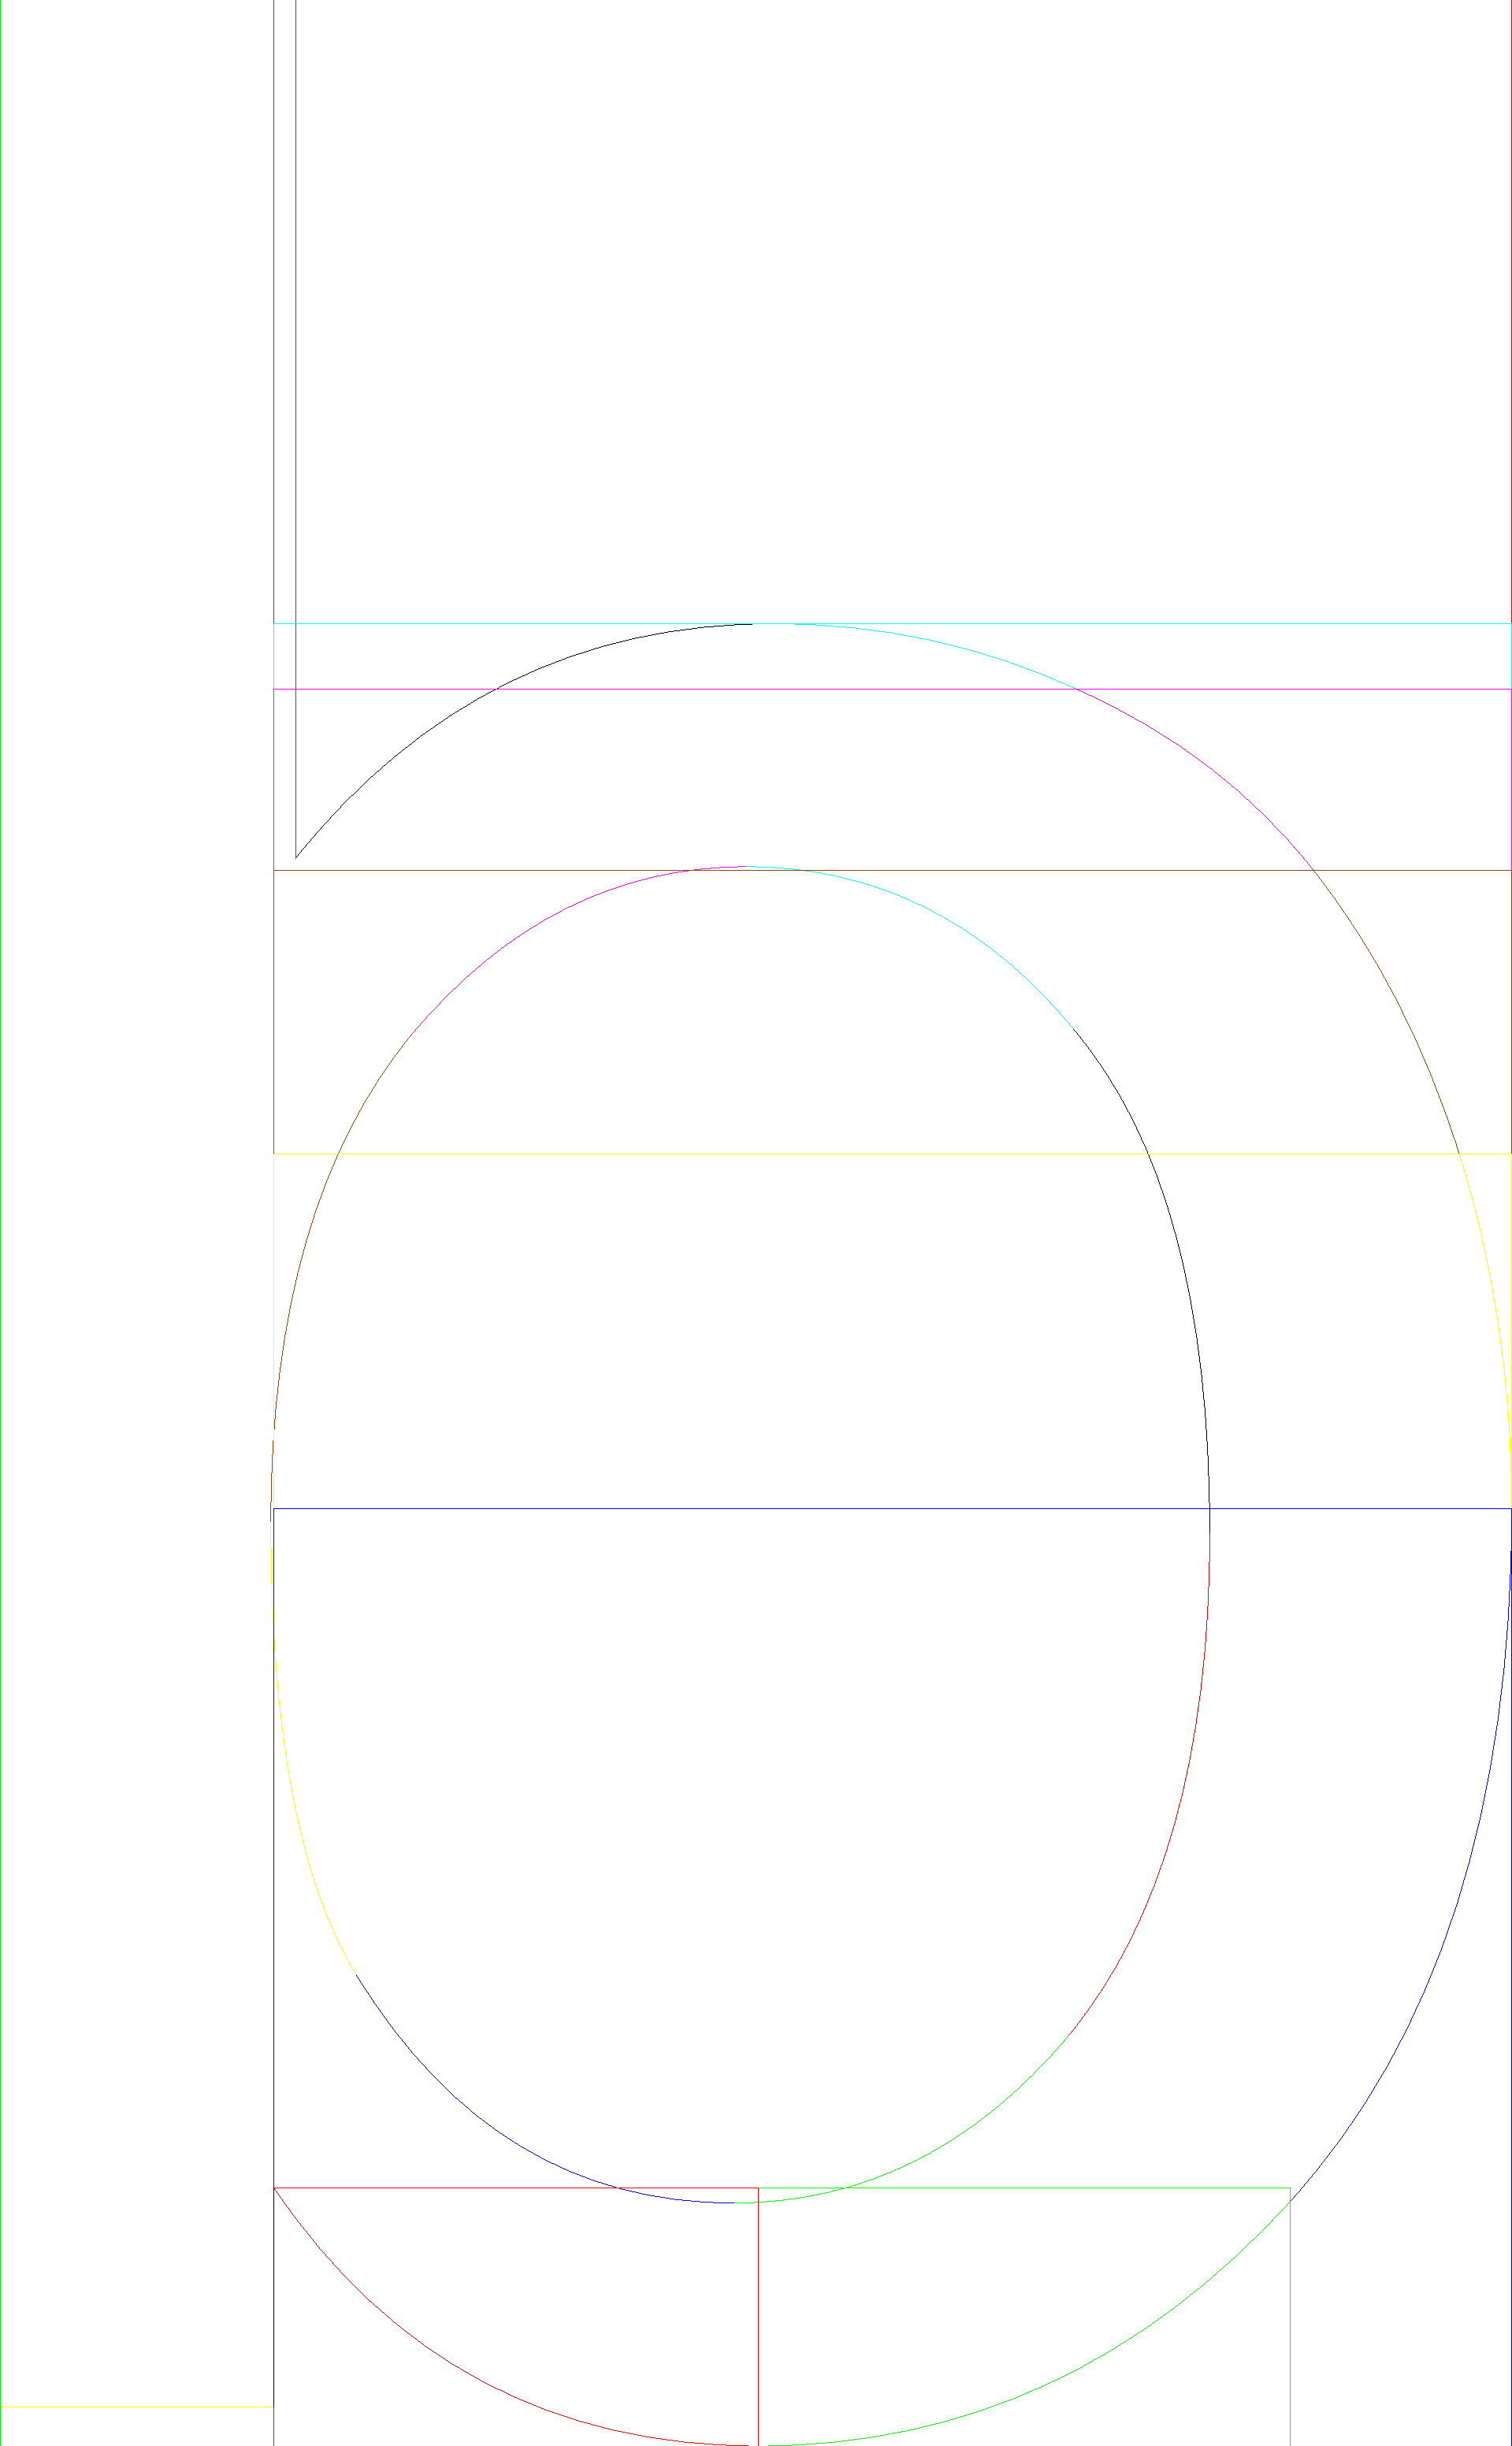
\includegraphics[height=12cm]{Ressources/pdf/b3.pdf}
    \caption{Construction pas à pas d'une « bounding box »}
    \label{Bounding box b}
  \end{center}
\end{figure}

\medskip

Enfin, on a calculé, pour différents documents, la fréquence d'apparition des caractères étudiés, pour pondérer les aires.

\medskip

\newpage

\noindent \textbf{Aspects graphiques}

N.B. : On a préféré produire les figures de ce document avec Ocaml plutôt que Caml Light pour pouvoir les exporter en \textsc{pdf}. Cela a demandé la réécriture de certaines fonctions et des conversions manuelles.

\medskip

Une cubique de Bézier est construite efficacement par l'algorithme de De Casteljau, ce qui en justifie l'utilisation. Ci-dessous, on construit une suite de barycentres, et le barycentre $P_{ttt}$ est sur la courbe.

\begin{figure}[h]
  \begin{center}
    \begin{tabular}{cc}
      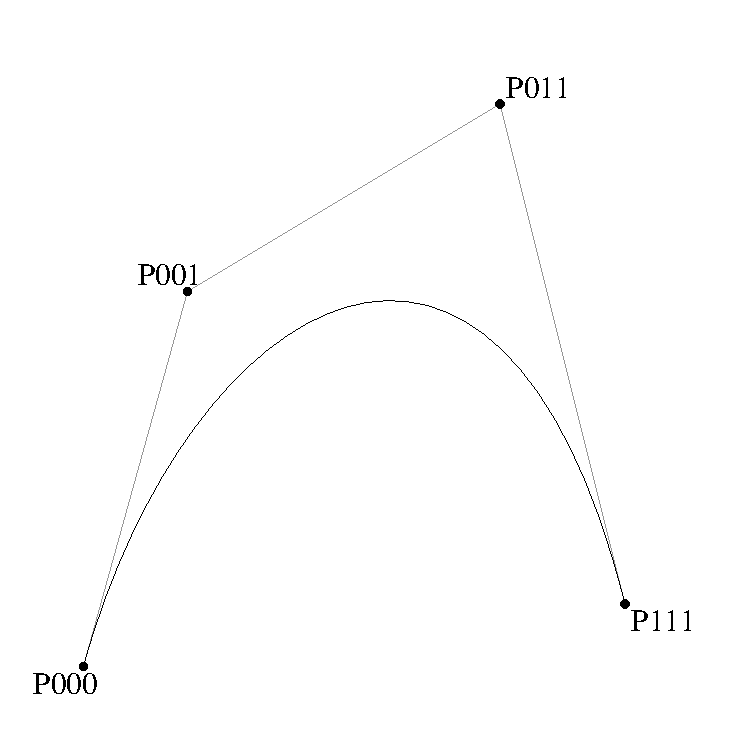
\includegraphics[height=6cm]{Ressources/pdf/f1.pdf} &
      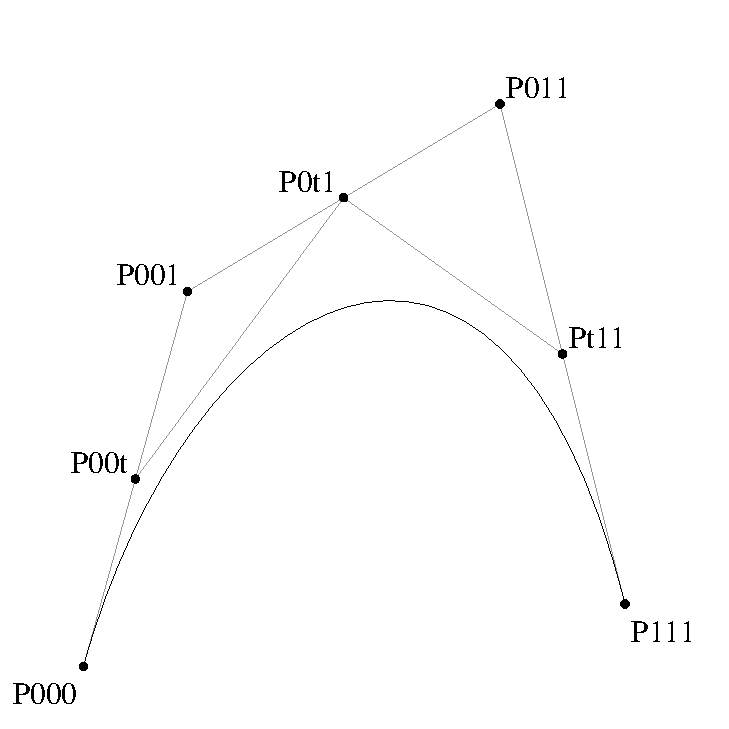
\includegraphics[height=6cm]{Ressources/pdf/f2.pdf} \\
      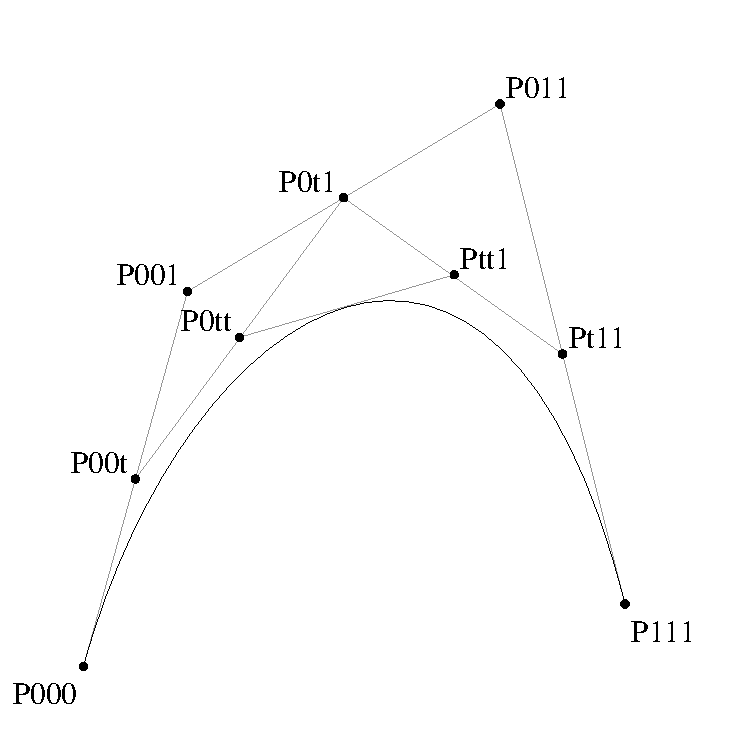
\includegraphics[height=6cm]{Ressources/pdf/f3.pdf} & 
      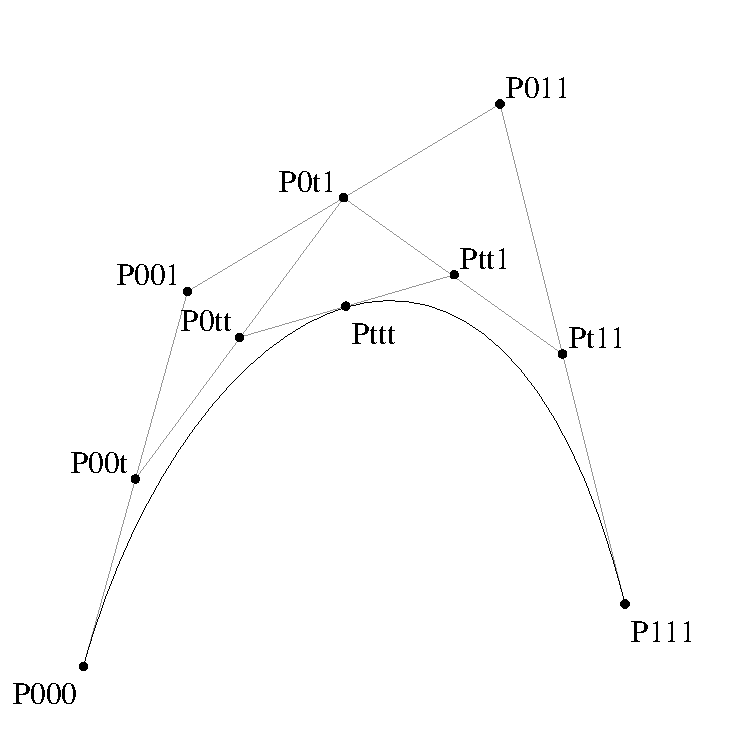
\includegraphics[height=6cm]{Ressources/pdf/f4.pdf} \\
    \end{tabular}
    \caption{Une étape de l'algorithme de De Casteljau}
  \end{center}
\end{figure}

\medskip

Les propriétés des cubiques de Bézier permettent d'écrire en oblique, et d'effectuer des rotations.

\begin{figure}[h]
  \begin{center}
    
\includegraphics[height=3cm]{Ressources/Images/TimesNewRoman.png}
    \caption{Texte en Times New Roman, penché de $0.1$ radians, obtenu avec Caml Light}
  \end{center}
\end{figure}

\pagebreak

\subsection{Restitution des résultats}

On donne les fréquences d'apparition calculées pour deux documents.

\medskip

\begin{figure}[h]
  \begin{center}
    \begin{tabular}{c|c|c}
      \diagbox{Lettre}{Document} & La Bête Humaine\footnote{La Bête Humaine, Émile Zola, 1890} & Thèse L. de Broglie\footnote{Recherche sur les quanta, Louis de Broglie, 1924} \\
      \hline \\
      e & 15.9 \%& 16.2 \% \\
      \hline \\
      a & 8.68 \% & 6.26 \% \\
      \hline \\
      i & 7.08 \% & 6.37 \% \\
      \hline \\
      t & 7.04 \% & 6.93 \% \\
      \hline \\
      s & 6.98 \% & 7.32 \% \\
      \hline \\
      r & 6.23 \% & 5.92 \% \\
      \hline \\
      o & 4.55 \% & 6.03 \% \\
    \end{tabular}
  \end{center}
  \caption{Fréquences d'apparition}
  \label{Fréquences d'apparition}
\end{figure}

{\scriptsize \noindent
  $^1$ La Bête Humaine, Émile Zola, 1890  \\
  $^2$ Recherche sur les quanta, Louis de Broglie, 1924
}

\medskip

La hauteur du \emph{x} permet de calculer les aires pondérées relatives suivantes.

\medskip

\begin{figure}[h]
  \begin{center}
    \begin{tabular}{c||c|c|c}
      Hauteur du x & \diagbox{Fonte}{Document} & La Bête Humaine & Thèse L. de Broglie \\
      \hline \\
      1062 & Arial & 0.377 & 0.399 \\
      \hline \\
      1120 & DejaVu Sans & 0.364 & 0.385 \\
      \hline \\
      916 & Times & 0.363 & 0.386 \\
      \hline \\
      409 & Garamond & 0.356 & 0.370 \\
      \hline \\
      1149 & Comic Sans MS & 0.351 & 0.374 \\
      \hline \\
      866 & Courier New & 0.320 & 0.330 \\
    \end{tabular}
  \end{center}
  \caption{Aires pondérées relatives}
  \label{Aires pondérées relatives}
\end{figure}

\subsection{Analyse – Exploitation – Discussion}

La \textsc{Figure} \ref{Fréquences d'apparition} met en évidence les importantes fluctuations d'un document à un autre. C'est pourquoi on ne peut pas facilement généraliser les résultats de la \textsc{Figure} \ref{Aires pondérées relatives}.

D'autre part, aucune fonte ne semble se démarquer des autres, si ce n'est \emph{Courier New}, qui présente cependant l'inconvénient de consommer plus de papier avec sa chasse fixe, et est peu lisible.

\section{Conclusion générale}

Les glyphes des fontes PostScript Type 1 sont efficacement décrites à l'aide des cubiques de Bézier.

L'étude de ces glyphes, par la manipulation de ces objets mathématiques, permet de conclure que le choix d'une fonte d'écriture n'est pas un paramètre d'influence remarquable sur les coûts d'impression.

Il vaut ainsi mieux se préoccuper de la lisibilité et de l'esthétique, ainsi que du coût d'entretien d'une imprimante, plutôt que du choix de fonte à adopter.

\section{Références bibliographiques additionnelles}

Aucune référence supplémentaire à mentionner.

\end{document}
